\documentclass[12pt,a4paper]{article}
  \usepackage[latin1]{inputenc}
  \usepackage[T1]{fontenc} 
  \usepackage[francais, english]{babel} 
  \usepackage{amsmath, amsthm}
  \newtheorem{theorem}{Theorem}
\newtheorem{proposition}{Proposition}
\newtheorem{lemma}{Lemma}
\newtheorem*{proof*}{Proof}
\newtheorem{definition}{Definition}

\newtheorem{exercise}{Exercise}
\newtheorem{question}{Question}

\newtheorem{example}{Example}

\newtheorem{remark}{Remark}

\usepackage[a4paper,left=2cm, right=2cm,top=3cm,bottom=3cm]{geometry}
\usepackage{cancel}
\usepackage{bm}
  \usepackage{amssymb,amsfonts}
  \usepackage{mathrsfs}
  \usepackage{color}
  %\usepackage{hyperref}
	\usepackage{dsfont}
	\usepackage{graphicx}
	\usepackage{algorithmicx}
    \usepackage[ruled]{algorithm}
    \usepackage{algpseudocode}
     \usepackage{marginnote}
\newcommand{\Ptr}{\mathcal P^{\rm tr}}
\newcommand{\tr}{{\rm tr}}
\newcommand{\N}{\mathbb N}
\newcommand{\calN}{\mathcal N}
\newcommand{\bP}{\bold P}
\newcommand{\calK}{\mathcal K}
\newcommand{\calF}{\mathcal F}
\newcommand{\calH}{\mathcal H}
\newcommand{\calP}{\mathcal P}
\newcommand{\calC}{\mathcal C}
\newcommand{\R}{\mathbb R}
\newcommand{\Ktr}{\calK^{\rm tr}}
  \title{ \bfseries \Huge {Stochastic processes}} 
  \author{  \scshape  Amina Benaceur }
 \date{\today}       
  \sloppy         
  \newcommand\red[1]{\textcolor{red} {#1} }
  \begin{document}
  \maketitle
  \section{Preliminaries}
  Probability theory studies random phenomena. 
  When observing a random phenomenon, the set of possible outcomes $\omega$ lies in a sample space $\Omega$. 
  For technical reasons, the collection of events $\calF$ assigned a probability is larger than the collection of all subsets of $\Omega$, i.e.
  \begin{itemize}
  	\item The impossible event $\emptyset$ and the certain event $\Omega$ are in $\calF$;
  	\item If $A$ is in $\calF$, the so is $\bar A$;
  	\item The union of events in $\calF$ is also in $\calF$.
  \end{itemize} 
  
  
  \subsection{Random variables}
  A random variable (rv) is roughly speaking a numerical quantity that takes random values.
  Consider a set of students $s_1, s_2,\ldots, s_n$ in this class. 
  We record their sleep time that we denote $X$. 
  $X$ is a random function that takes different random values for each student.
  We can do the same for their wake up time $W$.
  Wa plug in the student to the function, and get the numerical value $x$ or $Y$.
  $X$ and $Y$ are abstract object/quantity whose value is determined once we know the outcome of the experiment.
  \begin{definition}
  	A random variable is a function $X: \Omega \rightarrow \R$ such that for all $a\in\R$, the event $\{X\leq a\} = \{\omega; X(\omega)\leq a\}$ can be assigned a probability, that is, $\{X\leq a\} \in\calF$.
  	A function $X$ for which $E$ is denumerable is called a discrete random variable if for all $x\in E$, $\{X = x\}\in\calF$.
  	\end{definition}
In plain words, a random variable is a variable whose possible values are numerical outcomes of a random phenomenon. There are two types of random variables, discrete and continuous.
\begin{itemize}
	\item A discrete random variable is one which may take on only a countable number of distinct values. 
	Discrete random variables are usually counts.
	If a random variable can take only a finite number of distinct values, then it must be discrete. 
	Examples of discrete random variables include 
	\begin{enumerate}
	\item The number of children in a nuclear family;
	\item The number of students in an on-campus food truck;
	\item A prayer attendance at the UM6P mosque;
	\item The number of professors in a department.
	\end{enumerate}
	%the number of children in a family, the Friday night attendance at a cinema, the number of patients in a doctor's surgery, the number of defective light bulbs in a box of ten.
	The probability distribution (or probability mass function) of a discrete random variable is a list of probabilities associated with each of its possible values. 
	\item  A continuous random variable is one which takes an infinite number of possible values. Continuous random variables are usually measurements. 
	
	Examples of continuous random variables include 
	\begin{enumerate}
		\item Height;
		\item Weight;
		\item Water flow rate in a sink.
	\end{enumerate}
	Examples include height, weight, the amount of sugar in an orange, the time required to run a mile.
\end{itemize}
\begin{remark}
	\begin{enumerate}
		\item Several rvs can be defined on the same sample space.
		\item A function of one or more rvs is also an rv.
	\end{enumerate}
\end{remark}
If $X$ is a discrete r.v., then thefinite or countably in?nite set of values x such that $P (X = x) > 0$ is called the
support of $X$.
Discrete random variables have a probability mass function (PMF) which gives the probability of an event $X=a$ as $P(X=a)$.
Note that this is positive if $x$ is in the support of $X$, and $0$ otherwise.
The support of a discrete r.v. is a set of integers.
In contrast, a continuous r.v. can take on any real value in an interval (possibly even the entire real line).

\begin{example}
	\begin{enumerate}
		\item Consider $X$ to be the outcome of a fair coin toss.
		What is the support of $X$? What is $P(X=H)$ and $P(X=T)$?
		\item Consider $Y$ to be the outcome of a fair die roll. What is the support of $Y$. What is $P(Y=6)$ and $P(Y=T)$?
	\end{enumerate}
\end{example}
\begin{theorem}[Valid PMFs]. Let $X$ be a discrete r.v. with support $x_1, x_2, \dots$
	(assume these values are distinct and, for notational simplicity, that the support is countably infinite; the analogous results hold if the support is finite). 
	The PMF $p_X$
	of $X$ must satisfy the following criteria:
	\begin{enumerate}
		\item Nonnegative: $p_X (x) > 0$ if $x$ is in the support of $X$ and $p_X(x) = 0$ otherwise;
		\item Sums to $1$: $\sum_{j=1}^{\infty} p_X(x_j ) = 1$.
	\end{enumerate}
\end{theorem}
For continuous variables $P(X=a) = 0$.

All random variables (discrete and continuous) have a cumulative distribution function (CDF). 
It is a function giving the probability that the random variable $X$ is less than or equal to $x$, for every value $x$, i.e., $F_X: x\mapsto P(X\leq x)$. 
For a discrete rv, the cumulative distribution function is found by summing up the PMF, i.e., $\sum_{x_k\leq x} p(x_k)$.
Fo a continuous rv, it is given by intergrating the PDF, i.e. $\int_{-\infty}^x f$.

\begin{exercise}
	\begin{enumerate}
		\item Benford?s law states that in a very large variety of real-life data sets, the first digit
		approximately follows a particular distribution with about a $30\%$ chance of a $1$, an $18\%$
		chance of a $2$, and in general
		\begin{equation}
			P (D = j) = log_{10}\left(\frac{j+1}j\right),\quad\forall j \in \{1,2,3,\ldots,9\},
		\end{equation}
		where D is the first digit of a randomly chosen element. Check that this is a valid PMF.
	\end{enumerate}
\end{exercise}
	
\subsection{Bernoulli, binomial, exponential, Indicator rv, Poisson}
Some distributions have so many applications that they have
their own names.

We start with a very simple but useful case: an r.v. that can take on only two possible values, 0 and 1.
\begin{definition}[Bernoulli distribution]. 
	An r.v. $X$ is said to have the Bernoulli distribution with parameter $p$ if $P (X = 1) = p$ and $P (X = 0) = 1-p$, where $0<p<1$. We write this as $X \sim {\rm Bern}(p)$. The symbol $\sim$ is read "is distributed as".
\end{definition}
We often imagine Bernoulli rvs using coin tosses, with $X=1$ if heads and $X=0$ if tails.
An experiment that can result in either a "success"
or a "failure" is called a Bernoulli trial. 
A Bernoulli rv can be thought of as the indicator of success in a Bernoulli trial: it equals $1$ if the trial succeeds and $0$ if the trial fails.
The parameter $p$ is generally called the success parameter or the probability of success.

Imagine the case where we have a set of $n$ independent Bernoulli trials with the same parameter $p$, a coin toss as an example.
Let $X$ be the number of successes. The distribution of $X$ is called the binomial distribution with parameters $n$ and $p$. We thus write $X\sim{\rm Bin}(n,p)$.
Note that both the Bernoulli and the binomial distributions can be connected to the stories/experiments that initiated them. 
It is good to keep them in mind to develop intuition that often eases problem solving.
\begin{proposition}
	The PMF of a binomial distribution ${\rm Bin}(n,p)$ is 
	\begin{equation}
		P(X=k) = \left(^k_n\right) p^k (1-p)^{n-k}
	\end{equation}
	for $0\leq k\leq n$, and $0$ for $k>n$.
\end{proposition}
\begin{definition}[Binomial distribution]. 
	An r.v. $X$ is said to have the Bernoulli distribution with parameter $p$ if $P (X = 1) = p$ and $P (X = 0) = 1-p$, where $0<p<1$. We write this as $X \sim {\rm Bern}(p)$. The symbol $\sim$ is read "is distributed as".
\end{definition}

\begin{exercise}
	Let $X \sim {\rm Bin(n, p)}$, and $q = 1-p$.
	\begin{enumerate}
		\item What is $p$ in terms of probability? (probability of failure)
		\item We introduce the rv $Y = n-X$. What is the PMF of $Y$ ($Bin(n, q)$)?
	\item Independent Bernoulli trials are performed, with probability $1/2$ of success, until
	there has been at least one success. Find the PMF of the number of trials performed.
	\item Independent Bernoulli trials are performed, with probability $1/2$ of success, until there has been at least one success and at least one failure. 
	Find the PMF of the number of trials performed.
	\end{enumerate}
\end{exercise}

\subsection{Probability inequalities}
The Cauchy-Schwarz inequality is one of the most famous inequalities in all of mathematics. Its probabilistic form is as follows
\begin{theorem}[Cauchy-Schwarz]
	For any r.v.s $X$ and $Y$ with finite variances,
	\begin{equation}
		|E[XY]| \leq \sqrt{E[X^2]E[Y^2]}.
	\end{equation}
\end{theorem}
\begin{proof}
	\begin{equation}
		\forall t\in\R, \quad 0\leq E[Y-tX]^2 = E[Y^2]-2tE[XY]+t^2E[X^2]
	\end{equation}
	Differentiate with respect to $t$ and see where the minimum is.
\end{proof}
\begin{example}
	Let $X,Y$ be two rvs such that $E[X]=E[Y]= 0$.
	Prove that $-1\leq cov(X,Y)\leq 1$.
\end{example}
\begin{theorem}[Markov inequality]
	For any rv $X$ and a constant $a>0$
	\begin{equation}
		P(X>a)\leq\frac{E[X]}{a}
	\end{equation}
\end{theorem}
For an intuitive interpretation, let $X$ be the age of a randomly selected individual from a population. 
Taking $a = 2E[X]$, Markov?s inequality says that
$P (X \geq 2E[X]) \leq 0.5$, 
i.e., it is impossible for more than half the population
to be at least twice the average age. 
This is clearly true, since if over half the population were at least twice the average age, those people would already drive the average above what it is.

Chebychev is a prominent Russian mathematician fom the 19th century.
\begin{theorem}[Chebychev inequality]
	Let $X$ be an rv with mean $\mu$ and variance $\sigma^2$.
	\begin{equation}
		\forall a>0, \quad P(|X-\mu|\geq a)\leq\frac{\sigma^2}{a^2}
	\end{equation}
\end{theorem}
\begin{proof}
	Markov's property yields 
	$$
		P\left((X-\mu)^2>a^2\right)\leq\frac{E[(X-\mu)^2]}{a^2}.
	$$
	$P\left((X-\mu)^2>a^2\right) = P\left(|X-\mu|>a\right)$ and $E[(X-\mu)^2] = \sigma^2$, whereof the result.
\end{proof}
For $a = c\sigma$,  $c > 0$, we get
$$
P (|X-\mu| \geq c\sigma) \leq c^2.
$$
To get an intuition of the inequality, it gives us an upper bound on the probability of an r.v. being more than $c$
standard deviations away from its mean, e.g., there can't be more than a 25\% chance of being 2 or more standard deviations from the mean.



\subsection{Limit theorems}
Let $X_1,\ldots, X_n$ be i.i.d random variables with mean $\mu$ and variance $\sigma^2$. 
Let 
$$\bar X_n = \frac{X_1+X_2+\ldots+X_n}{n}.$$
The variance of $\bar X_n$ is $\sigma^2/n$. 
\subsubsection{Weak Law of large numbers (WLLN)}
\begin{theorem}
For $n\geq 1$, and i.i.d random variables $X_1,\ldots, X_n$ with finite variance, it holds that
\begin{equation}
\forall \epsilon\geq 0,\qquad \underset{n\rightarrow\infty}{lim}	\text{Pr}\left\{\left|\left(\bar X_n-\mu\right)\right|\geq\epsilon\right\} = 0.
\end{equation}
\end{theorem}

\begin{proof}
	Using Chebychev inequality, we get
	$$
	Pr\left(\left|\bar X_n-\mu\right|\geq \epsilon\right)
	\leq  \frac{\sigma^2}{n\epsilon^2}\underset{n\rightarrow\infty}{\rightarrow}0.
	$$
\end{proof}
Every time we use the proportion of times that something happened as an approximation to its probability, we are implicitly appealing to the LLN. 
Every time we use the average value in the replications of some quantity to approximate its theoretical average, we are implicitly appealing to the LLN.

\begin{remark}
	[LLN does not contradict the memoryless property]. In the above exam-
	ple, the law of large numbers states that the proportion of Heads converges to 1/2,
	but this does not imply that after a long string of Heads, the coin is due? for a Tails
	to balance things out. Rather, the convergence takes place through swamping: past
	tosses are swamped by the infinitely many tosses that are yet to come
\end{remark}

\subsubsection{Central limit theorem (CLT)}
The law of large numbers says that as $n\rightarrow\infty$, $\bar X_n$ converges to the constant $\mu$ (with probability 1). But what is its distribution along the way to becoming a constant? This is addressed by the central limit theorem (CLT).
The CLT states that for large n, the distribution of $\bar X_n$ after standardization approaches a standard normal distribution $\calN(0,1)$. 
By standardization, we mean that we subtract $\mu$, the expected value of $\bar X_n$, and divide by $\sigma/\sqrt{n}$, the standard deviation of $\bar X_n$.


\begin{theorem}[Central limit theorem]
	Let $X_1,\ldots, X_n$ be i.i.d random variables with finite mean $\mu$ and finite variance $\sigma^2$. It holds that
	\begin{equation}
		\underset{n\rightarrow\infty}{lim}\text{Pr}\left\{\frac{\bar X_n-\mu}{\sigma\sqrt{n}}\leq z\right\} = \calN(0,1)(z)
	\end{equation}
	which is referred to as convergence in distribution
\end{theorem}
Let?s take a moment to admire the generality of this result. 
The distribution of the individual $X_i$ can be anything in the world, as long as the mean and variance are finite. 
We could have a discrete distribution like the Binomial, a bounded distribution like the Beta, or a distribution with multiple peaks and valleys. 
No matter what, the act of averaging will cause Normality to emerge. 
	
This does not mean that the distribution of the Xj is irrelevant, however. 
If the $X_i$ have a highly skewed or multimodal distribution, we may need n to be very large before the Normal approximation becomes accurate; at the other extreme, if the $X_i$ are already i.i.d. Normals, the distribution of $\bar X_n$ is exactly $\calN (\mu, \sigma^2/n)$ for all $n$. 

\newpage
\subsection{Stochastic processes}
\begin{definition}
	We give two definitions
	\begin{itemize}
		\item 
		A stochastic process is a sequence of random variables with values in a set $E$ indexed by time.
		The space $E$ is called a state space. $E$ is a countable space. 
		\item A stochastic process is a probability distribution over a set of paths
	\end{itemize}
	\end{definition}
\paragraph{Examples:}
\begin{enumerate}
	\item Discrete-time stochastic process $(X_i)_{1\leq i\leq n}$. If $X_n = i$, then the process is said to be in state $i$ at time $n$.
	\item Continuous time stochastic-process $(X_t)_{t\geq 0}$.
\end{enumerate}
\paragraph{Exercice}
For two positive integers \( A \) and \( B \), what is the probability that the random walk reaches \( A \) before it reaches \( -B \)? Let \( \tau \) be the first time at which the random walk reaches either \( A \) or \( -B \). Then \( X_\tau = A \) or \( -B \).

Define
$$
f(k) = P(X_\tau = A \mid X_0 = k),
$$
and note that our goal is to compute \( f(0) \). The recursive formula
$$
f(k) = \frac{1}{2} f(k+1) + \frac{1}{2} f(k-1)
$$
follows from considering the outcome of the first coin toss. We also have the boundary conditions
$$
f(A) = 1, \quad f(-B) = 0.
$$
If we let \( f(-B+1) = \alpha \), then it follows that
$$
f(-B + r) = \alpha^r \quad \text{for all} \quad r \leq A + B.
$$
Therefore, \( \alpha = \frac{B}{A + B} \), and it follows that
$$
f(0) = \frac{B}{A + B}.
$$


	
\paragraph{Examples of stochastic processes}

\subsubsection{Random walk}
Consider a set of i.i.d variables $Y_1,\ldots, Y_n$ where for each variable $Y_k$, $k\in\{1,\ldots, n\}$, $Y_k\in\{-1,1\}$ with equal probability. $X_1,X_2,X_3,\ldots$ is a stochastic process, and we introduce a random walk as 
\begin{equation}
	X_N = Y_1+Y_2+\ldots+ Y_N. 
\end{equation}
%The random walk is usually used to model the trajectory of people under substances that momentarily annihilate their mental capabilities.

By the central limit theorem, we know that for a large enough integer $n$, the
distribution of $\frac{1}{\sqrt{n}} X_n$ converges to the normal distribution with mean 0 and
variance 1. This already tells us some information about the random walk.
We state some further properties of the random walk

\begin{proposition}
	The following statements hold true
	\begin{enumerate}
	\item $\forall k\geq 0, \ E[X_k] = 0$.
	\item The random walk has independent increments, i.e., $\forall\ 0 = k_0 \leq k_1 \leq\ldots\leq k_r$, the r.v.s $X_{k_i+1}-X_{k_i}$ for $0 \leq i \leq r-1$ are mutually independent.
	\item The random walk is stationary, i.e., $\forall, k,h\geq 0$, the distribution of $X_{k+h}-X_k$ is the same as the distribution of $X_h$.	
	\end{enumerate}
	\end{proposition}
	
\paragraph{Exercise:} A particle moves n steps on a number line. 
	The particle starts at 0, and at each step it moves 1 unit to the right or to the left, with equal probabilities. 
	Assume all steps are independent. 
	Let $Z$ be the particle?s position after $n$ steps. Find the PMF of $Z$. If k is an integer between ?n and n (inclusive) such that n+k is an even number, we get
	$$ P(Z = k) = \binom{n}{\frac{n+k}{2}}\left(\frac{1}{2}\right)^n$$
	otherwise $ P(Z = k) = 0$
	
	For two positive integers $A$ and $B$, what is the probability that the random walk reaches $A$ before it reaches $-B$?
	
		
		\subsection{Application to Fair Gambling Games}
		
		We took the high road for a while, but let's now discuss random walks in a more conventional setting?gambling.
		
		A gambler goes to Las Vegas with $n$ in her pocket. 
		Her plan is to make only $1$ bets and somehow she has found a casino that will offer her truly even odds; namely, she will win or lose $1$ on each bet with probability $\frac{1}{2}$. She'll play until she is broke or she has won $m$. In the latter case, she will go home with
		$$
		w = n + m
		$$
		dollars. What's the probability that she goes home a winner?
		
		This is identical to the flea problem that we just analyzed. Going broke is analogous to falling off the Cliff of Doom. Going home a winner is analogous to falling into the Pit of Disaster, just a lot more fun.
		
		Our analysis of Stencil's life tells us everything we want to know about the gambler's prospects:
		\begin{itemize}
			\item The gambler goes home broke with probability
			$$
			\frac{n}{n + m};
			$$
			\item The gambler goes home a winner with probability
			$$
			\frac{m}{n + m};
			$$
			\item The gambler goes home with probability
			$$
			\frac{n}{n + m} + \frac{m}{n + m} = 1;
			$$
			\item And the number of bets before the gambler goes home is expected to be
			$$
			n \cdot (w - n) = nm.
			$$
		\end{itemize}
		
		If the gambler gets greedy and keeps playing until she goes broke, then
		\begin{itemize}
			\item The gambler eventually goes broke with probability $1$, and
			\item The number of bets before the gambler goes broke is expected to be infinite.
		\end{itemize}
		
		The bottom line here is clear: when gambling, quit while you are ahead?if you play until you go broke, you will certainly go broke. And that's the good news!
		
		Matters get much worse for the more typical scenario where the odds are against you. Let's see why.
		
		\subsubsection{Gambler's Ruin}
		
		So far, we have considered unbiased random walks, where the probability of moving up or down (or left or right) is $\frac{1}{2}$. Unfortunately, things are never quite this simple (or fair) in real casinos.
		
		For example, suppose the gambler goes to Las Vegas and makes $1$ bets on red or black in roulette. In this case, she will win $1$ with probability
		$$
		\frac{18}{38} \approx 0.473
		$$
		and she will lose $1$ with probability
		$$
		\frac{20}{38} \approx 0.527.
		$$
		That's because the casinos add those bothersome green 0 and 00 to give the house a slight advantage.
		
		At first glance (or after a few drinks), $\frac{18}{38}$ seems awfully close to $\frac{1}{2}$ and so our intuition tells us that the game is "almost fair". So we might expect the analysis we just did for the fair game to be "?lmost right"? or the real game. For example, if the gambler starts with $100$ and quits when she gets ahead by $100$ in the fair game, then she goes home a winner with probability
		$$
		\frac{100}{200} = 0.5.
		$$
		And, if she wants to improve her chances of going home a winner, she could bring more money. If she brings $1000$ and quits when she gets ahead by $100$ in the fair game, then she goes home a winner with probability
		$$
		\frac{1000}{1100} \approx 0.91.
		$$
		
		So, given that the real game is "almost fair," we might expect the probabilities of going home a winner in these two scenarios to be "?lmost 50\% and 91\%,"? espectively.
		
		Unfortunately for the gambler, all this "almost" reasoning will almost surely lead to disaster. Here are the grim facts for the real game where the gambler wins $1$ with probability $\frac{18}{38}$.
		
		$$
		\text{For } n = 100, \text{ probability she reaches } n + 100 \text{ before } 0: \text{ 1 in 37649.619496...}
		$$
		$$
		\text{For } n = 1000, \text{ probability she reaches } n + 100 \text{ before } 0: \text{ 1 in 37648.619496...}
		$$
		
		Except on the very low end, the amount of money she brings makes almost no difference! She is almost certain to go broke before winning $100$. Let's see why.
		
		\subsubsection{Finding a Recurrence}
		
		We can approach the gambling problem the same way we studied the life of Stencil. Suppose that the gambler starts with $n$ dollars. She wins each bet with probability $p$ and plays until she either goes bankrupt or has $w = n + m$ dollars in her pocket. (To be clear, $w$ is the total amount of money she wants to end up with, not the amount by which she wants to increase her wealth, which is $m$.) Our objective is to compute $R_n$, the probability that she goes home a winner.
		
		As usual, we begin by identifying some boundary conditions. If she starts with no money, then she's bankrupt immediately so $R_0 = 0$. On the other hand, if she starts with $w$ dollars, then she's an instant winner, so $R_w = 1$.
		
		Now we divide the analysis of the general situation into two cases based on the outcome of her first bet:
		\begin{itemize}
			\item She wins her first bet with probability $p$. She then has $n + 1$ dollars and probability $R_{n+1}$ of reaching her goal of $w$ dollars.
			\item She loses her first bet with probability $1 - p$. This leaves her with $n - 1$ dollars and probability $R_{n-1}$ of reaching her goal.
		\end{itemize}
		
		Plugging these facts into the Total Probability Theorem gives the equation:
		$$
		R_n = p R_{n+1} + (1 - p) R_{n-1}.
		$$
		
		\subsubsection{Solving the Recurrence}
		
		Rearranging the terms in the equation gives us a recurrence for $R_n$, the probability that the gambler reaches her goal of $w$ dollars if she starts with $n$:
		$$
		R_0 = 0,
		$$
		$$
		R_w = 1,
		$$
		$$
		p R_{n+1} - R_n + (1 - p) R_{n-1} = 0 \quad (0 < n < w).
		$$
		
		The characteristic equation is:
		$$
		p x^2 - x + (1 - p) = 0.
		$$
		Using the quadratic formula, we get the roots:
		$$
		x = 1 \pm \frac{\sqrt{1 - 4p(1 - p)}}{2p}.
		$$
		If the gambler is equally likely to win or lose each bet, then $p = \frac{1}{2}$, and the characteristic equation has a double root at $x = 1$. This is the situation we considered in the flea problem. The general solution in this case is:
		$$
		R_n = a + b n.
		$$
		
		Suppose that the gambler is not equally likely to win or lose each bet; that is, $p \neq \frac{1}{2}$. Then the two roots of the characteristic equation are different, leading to the general solution:
		$$
		R_n = a \left( \frac{1 - p}{p} \right)^n + b\times 1^n.
		$$
		In mathematical terms, this is where the fair game and the ``almost fair'' game take off in completely different directions: in one case we get a linear solution and in the other we get an exponential solution! This is going to be bad news for anyone playing the ``almost fair'' game.
		
		Anyway, substituting the boundary conditions into the general form of the solution gives a system of linear equations:
		$$
		0 = a + b
		$$
		$$
		1 = a \left(\frac{1-p}{p} \right)^w + b
		$$
		Solving this system gives:
		$$
		a = \frac{1}{\left( \frac{1-p}{p} \right)^w - 1}, \quad b =- \frac{1}{\left(\frac{1-p}{p} \right)^w - 1}
		$$
		
		Substituting these values back into the general solution gives:
		$$
		R_n = \left(\frac{1}{\left( \frac{1-p}{p} \right)^w - 1}\right) \left( \frac{1-p}{p} \right)^n 
		- \frac{1}{\left( \frac{1-p}{p} \right)^w-1}
		$$
		Hence
		$$
		R_n = \frac{\left( \frac{1-p}{p} \right)^n-1}{\left(\frac{1-p}{p} \right)^w-1}
		$$
		
		(Suddenly, Stencil's life doesn't seem so bad, huh?)
		\paragraph{Bad news!}
		We have an answer! But it's not good news. If the gambler starts with $n$ dollars and wins each bet with probability $p$, then the probability she reaches $w$ dollars before going broke is:
		$$
		\frac{\left( \frac{1-p}{p} \right)^n-1}{\left(\frac{1-p}{p} \right)^w-1}
		$$
		Let's try to make sense of this expression. If the game is biased against her, as with roulette, then $1 - p$ (the probability she loses) is greater than $p$ (the probability she wins). If $n$, her starting wealth, is also reasonably large, then both exponentiated fractions are big numbers and the $-1$'s don't make much difference. Thus, her probability of reaching $w$ dollars is very close to:
		$$
		\left( 1 - \frac{1}{p} \right)^{n-w} = \left( 1 - \frac{1}{p} \right)^m
		$$
		In particular, if she is hoping to come out $m = 100$ dollars ahead in roulette, then $p = \frac{18}{38}$ and her probability of success is:
		$$
		\left( \frac{10}{9} \right)^{-100} = \frac{1}{37648.619496}
		$$
		This explains the strange number we arrived at earlier! In fact, this number does not change no matter how large $n$ gets, so even if the gambler starts with a trillion dollars, she is still not likely to ever get ahead by even $100$.
		
		\textbf{But Why?}
		
		Why does the gambler's starting wealth have so little impact on her probability of coming out ahead? Intuitively, there are two forces at work. First, the gambler's wealth has random upward and downward swings due to runs of good and bad luck. Second, her wealth has a steady, downward drift because she has a small expected loss on every bet. The situation is illustrated in Figure 20.2.
		
		\begin{figure}[h]
			\centering
			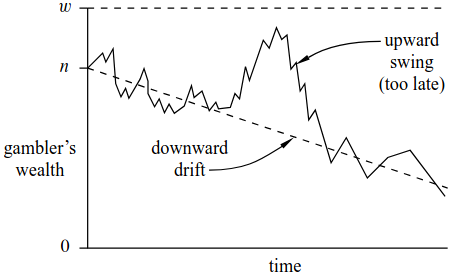
\includegraphics[width=0.6\textwidth]{images/drift_swing.png} 
			\caption{In a biased random walk, the downward drift usually dominates swings of good luck.}
		\end{figure}
		
		For example, in roulette, the gambler wins a dollar with probability $\frac{18}{38}$ and loses a dollar with probability $\frac{20}{38}$. Therefore, her expected return on each bet is:
		$$
		1 \times \frac{18}{38} + (-1) \times \frac{20}{38} = -\frac{2}{38} = -\frac{1}{19}
		$$
		Thus, her expected wealth drifts downward by a little over 5 cents per bet.
		
		One might think that if the gambler starts with a billion dollars, then she will play for a long time, so at some point she should have a lucky, upward swing that puts her $100$ ahead. The problem is that her capital is steadily drifting downward. And after her capital drifts down a few hundred dollars, she needs a huge upward swing to save herself. And such a huge swing is extremely improbable. So if she does not have a lucky, upward swing early on, she's doomed forever. As a rule of thumb, drift dominates swings over the long term.
		
	
	
	\subsubsection{ Expected Playing Time}
	
	Even though casino gamblers are destined to lose, some of them enjoy the process. So let?s figure out how long their enjoyment is expected to last. Let \( X_n \) be the expected number of bets before going home (broke or a winner).
	
	Reasoning as above, we can set up a recurrence for \( X_n \):
	\[
	X_0 = 0;
	\quad X_w = 0;
	\quad X_n = 1 + (1 - p) X_{n-1} + p X_{n+1}. \tag{20.3}
	\]
	This is the same as the recurrence for \( R_n \) in Equation 20.2 except for the inhomogeneous part.
	
	To find the particular solution, we try \( X_n = c \) (which doesn?t work) and then \( X_n = c + d n \) (which does work as long as \( p \neq \frac{1}{2} \)). Plugging \( X_n = c + d n \) into Equation 20.3 yields:
	\[
	c + d n = 1 + (1 - p)(c + d(n - 1)) + p(c + d(n + 1))
	\]
	\[
	= 1 + c + d n - (1 - p) d + p d n
	\]
	\[
	= 1 + c + d n - (1 - p) d + p d n.
	\]
	This simplifies to:
	\[
	c + d n = 1 + c + d n - (1 - p) d + p d n,
	\]
	and thus we find that
	\[
	d = \frac{1}{1 - 2p}.
	\]
	
	Since \( c \) is arbitrary, we will set \( c = 0 \) and our particular solution is
	\[
	X_n = \frac{n}{1 - 2p}.
	\]
	
	The characteristic equation for Equation 20.3 is
	\[
	p x^2 - x + (1 - p) = 0.
	\]
	We have already determined that the roots for this equation are
	\[
	\frac{1 - p}{p} \quad \text{and} \quad 1.
	\]
	
	Hence, the general solution to the recurrence is
	\[
	X_n = a \left( \frac{1 - p}{p} \right)^n + b + \frac{n}{1 - 2p}.
	\]
	
	Plugging in the boundary conditions, we find that
	\[
	0 = a + b;
	\]
	\[
	0 = a \left( \frac{1 - p}{p} \right)^w + b + \frac{w}{1 - 2p}. \tag{15}
	\]
	Thus,
	\[
	a =\frac{- \frac{w}{1 - 2p}}{ \left( \frac{1 - p}{p} \right)^w - 1},
	\]
	and
	\[
	b = \frac{\frac{w}{1 - 2p}}{ \left( \frac{1 - p}{p} \right)^w - 1}.
	\]
	
	The final solution to the recurrence is then
	\[
	X_n = \frac{-\left(\frac{w}{1 - 2p}\right) \left( \frac{1 - p}{p} \right)^n}{ \left( \frac{1 - p}{p} \right)^w - 1 }+\frac{ \left(\frac{w}{1 - 2p}\right)}{ \left( \frac{1 - p}{p} \right)^w - 1} + \frac{n}{ 1 - 2p}.
	\]
	wich leads to
	$$
	X_n = \frac{n}{ 1 - 2p} - \left(\frac{w}{1 - 2p}\right)\left[\frac{\left( \frac{1 - p}{p} \right)^n - 1 }{\left( \frac{1 - p}{p} \right)^w - 1 }\right]
	$$
	
	Yikes! The gambler won't have any fun at all if she is thinking about this equation. 
	Let's see if we can make it simpler in the case when \( m = w \, n \) is large. Since \( p < \frac{1}{2} \), \( \frac{1 - p}{p} > 1 \) and for large \( m \),
	\[
	\lim_{m \to \infty} \frac{w}{1 - 2p} \left[\frac{\left( \frac{1 - p}{p} \right)^n - 1 }{\left( \frac{1 - p}{p} \right)^w - 1 }\right] = \lim_{m \to \infty} \left(\frac{w}{1 - 2p} \right)\left(\frac{1 - p}{p} \right)^{-m}
	= 0.
	\]
	This means that as \( m \) gets large,
	\[
	X_n \sim \frac{n}{1 - 2p}.
	\]
	
	This is much simpler. It says that if the gambler starts with \( n \), she will expect to make about \( \frac{n}{1 - 2p} \) bets before she goes home broke. This seems to make sense since she expects to lose
	\[
	1 \times (1 - p) + (-1)\times p = 1 - 2p
	\]
	dollars on every bet, and she started with \( n \) dollars.
	
	
	
	
	
\newpage
\section{Discrete Markov chains}
\subsection{The Markov Property}
Let $X_n$ be a stochastic process with values in a countable state space $E$. $(X_n)$ is said to be a Markov chain (MC) if and only if
\begin{equation}\label{def:MC}
P(X_{k+1} = j \mid X_k = i, X_{k-1} = i_{k-1}, \dots, X_0 = i_0) = P(X_{k+1} = j \mid X_k = i),
\end{equation}
For convenience,~\eqref{def:MC} is often abbreviated as 
\begin{equation}\label{def:MC}
	P(X_{k+1} \mid X_k, X_{k-1} , \dots, X_0) = P(X_{k+1} \mid X_k),
\end{equation}
which means that the equality holds independently of sample values.
The property~\eqref{def:MC} is called the \textit{Markov property}.
Additionally, $(X_n)_{n\geq 0}$ is called a homogenous Markov chain (HMC) if the right-hand side of~\eqref{def:MC} is independent of $n$.
We introduce the probabilities $p_{ij}$ such that
\begin{equation}
	p_{ij} =  P(X_{n+1} = j \mid X_n = i)
\end{equation}
The matrix $\bold P = (p_{ij})_{i,j\in E}$ is the \textit{transition matrix}.
The elements of $\bP$ are probabilities. Therefore, they satisfy
\begin{equation}
	 \forall i,j\in E, \ p_{ij}\geq 0,\quad \text{and } \sum_{j \in E} p_{ij} = 1.
\end{equation}
\begin{definition}
	A \textit{Markov chain} is a discrete-time stochastic process $(X_k)_{k\geq 0}$ that satisfies the Markov property.
	\end{definition}
	In other words, a Markov chain is a stochastic process for which the sample values for each rv in $(X_k)_{k\geq 0}$ lie in a countable set $E$ and depend on the past only through the most recent rv $X_{k-1}$
	
	
	An HMC and its transition matrix $\bP$ are usually represented by a directed graph called a \textit{transition graph} $G$. 
	The nodes of $G$ are the states of the process. 
	$G$ has an oriented edge from node $i$ to node $j$ if and only if $p_{ij}>0$. 
	The transition probabilities $p_{ij}$ are inscribed on the corresponding oriented edge.
	The difference between zero and non-zero transition probabilities stands out clearly on a graph as edges are not represented until transition probabilities are non-zero.
	
\subsection{Classification of states}
\begin{definition}
	\begin{enumerate}
		\item An n-step walk is an ordered set of nodes $(i_0,\ldots,i_n), n\geq 1$, for which there is a directed edge from $i_{k-1}$ to $i_k$ for each $k\in\{\{1,\ldots,n\}\}$.
		\item A path is a walk in which no nodes are repeated
		A cycle is a walk in which the first and last nodes coincide.
		\item A state $j$ is accessible from $i$ f there is a walk from $i$ to $j$
		\item Two distinct states $i$ and $j$ communicate (denoted $i \leftrightarrow j$) if $i$ is accessible from $j$ and vice versa.
		\item A class is a non-empty set of states such that: $\forall i\in\calC,\ \forall j\neq i\in\calC$, if $i\leftrightarrow j$, then $j\in\calC$, and if  $i\cancel\leftrightarrow j$, then $j\notin\calC$.
		\item For finite-state Markov chains, a recurrent state is a state $i$ that is accessible from $i$ ($i$ is recurrent if $i\rightarrow j$ implies that $j\leftarrow i$
		\item A transient state is a state that is not recurrent.
		\item The period $d(i)$ of a state $i$ the greatest common divisor (gcp) of those values of $n$ for which $P^n_{ii}$. If the period is $1$, the state is aperiodic, and if the period is $2$ or more, then the state is periodic.
	\end{enumerate}
\end{definition}	
	\begin{question}
		What is the maximum number os steps in a path?
		What mathematical property?
		
		What is the probability to return to a recurrent state on the long run?
	\end{question}
	
	\begin{theorem}
	For finite-state MC, a class either consits exclusively of recurrent states, or consists exclusively of recurrent states	
	\end{theorem}
	
	
	\begin{theorem}
		For a MC, all states in the same class have the same period.	
	\end{theorem}
	\begin{definition}
		For a finite-state MC, an ergodic class of states is a class that is both recurrent and aperiodic. A MC consisting entirely of one ergodic class is called an ergodic chain.
	\end{definition}

	
\subsection{Distribution of an HMC}
The rv $X_0$ is called the initial state. From Bayes' rule
\begin{equation}
	P(X_0 = i_0, \ldots, X_k = i_k) = P(X_0 = i_0) P(X_1 = i_1 \mid X_0 = i_0)\ldots P(X_k = i_k \mid X_{k-1} = i_{k-1})
\end{equation}
Denoting the probability distribution of the initial state as $v(i_0) = P(X_0 = i_0)$, we obtain  
\begin{equation}
	P(X_0 = i_0, \ldots, X_k = i_k) = v(i_0) p_{i_0i_1} p_{i_1i_2}\ldots p_{i_{k-1}i_k}
\end{equation}
which constritutes the distribution of the HMC.
\begin{theorem}
The distribution of a discrete-time HMC is determined by its initial distribution and its transition matrix.	
	\end{theorem}
	
\subsection{Properties of Markov chains}
\subsection{Communicating classes}
\subsection{Stationarity and the steady state}

\begin{definition}
	A probability distribution satisfying 
	\begin{equation}
		 {\bm\pi} \bP  = {\bm\pi}
	\end{equation}
	is called a \textit{stationary distribution} of the transition matrix $\bP$. It can also be called a stationary distribution of the corresponding HMC.
\end{definition}


\begin{proposition}
	Let $\pi$ be a stationary distribution for $(X_n)_{n\geq0}$. 
	$\forall n \geq 0, \forall x \in E,\ \text{Pr}(X_n = x) = \pi(x)$, i.e., if thprobability distribution of the initial state $X_0$ is $\pi$, then for any $n\geq 0$, the probability distribution of $X_n$ is also $\pi$.
\end{proposition}

\begin{proposition}
	If a Markov chain is defined over a finite state space $E$, then it admits a stationary distribution
	\end{proposition}
	\begin{proof}
		Perron-Frobenius theorem
	\end{proof}


\begin{proposition}
	If a Markov chain chain is irreducible then all states are recurrent.
\end{proposition}
	
	
\begin{proposition}
	If a Markov chain chain is irreducible with finitely many states and aperiodic, then
	\begin{enumerate}
		\item It has a stationary distribution.
		\item The stationary distribution is unique.
		\item $s_i = \frac{1}{r_i}$, where $r_i$ is the expected time to return to state $i$. 
	\end{enumerate}
\end{proposition}
	
	
	\begin{exercise}
		Find the stationary distribution for some Markov chains
		\end{exercise}
		
	\begin{definition}
		A Markov chain with transition matrix $\bP$ on $E$ is irreducible if, for all $x, y \in E$, there exist $n \geq 1$ and $x = x0, x_1, . . . , x_n = y$ such that $P(x_0, x_1) \ldots P(x_{n?1}, x_n) > 0$.
		\end{definition}
	
\subsection{Periodicity}
If self-transition, then the MCis not periodic

Eyballing is not always sufficient



\subsection{Time reversal}

\subsection{Chapman-Kolmogorov equation}
\begin{theorem}
	$$
	P_{ij}(n+m) = \sum_{k=1}^n P_{ik}(n) P_{kj}(m)
	$$
\end{theorem}
\begin{proof}
	\begin{equation}
		\begin{alignedat}{2}
			P_{ij}(n+m) &= P(X_{n+m} = j|X_0 = i)\\
			&= \sum_{k=1}^n P(X_{n+m} = j \cap  X_n = k|X_0 = i)\\
			&= \sum_{k=1}^n P(X_{n+m} = j |X_0 = i\cap  X_n = k) P(X_n = k |X_0 = i)\\
			&= \sum_{k=1}^n P(X_{n+m} = j | X_n = k) P(X_n = k |X_0 = i)\\
			&= \sum_{k=1}^n P(X_{m} = j | X_0 = k) P(X_n = k |X_0 = i)\\
			&= \sum_{k=1}^n P_{kj}(m) P_{ik}(n), 
		\end{alignedat}
	\end{equation}
	wherof the result.
\end{proof}

\begin{definition}
	As stochastic process is reversible if and only if 
	\begin{equation}\label{def:rev}
		\pi(x){\rm Pr}(x, y) = \pi(y){\rm Pr}(y, x)
	\end{equation}
	A Markov chain $X$ is reversible with respect to a probability measure $\pi$ if its transition matrix is reversible with respect to $\pi$.
	\begin{proposition}\label{prop:rev}
		If a stochastic matrix $\bP$ is reversible with respect to a probability measure $\pi$, then $\pi$ is a stationary probability measure for $\bP$.
	\end{proposition}
	Proposition~\ref{prop:rev} is derived by summing~\eqref{def:rev} over $x \in E$.
	
\end{definition}

\newpage
\section{The Bernoulli process}

Here is an alternative description of the Bernoulli process:
\begin{enumerate}
	\item Start with a sequence of independent geometric random variables $T_1, T_2, \dots$, with common parameter $p$, and let these stand for the interarrival times.
	\item Record a success (or arrival) at times $T_1, T_1 + T_2, T_1 + T_2 + T_3, \dots$.
\end{enumerate}


\subsection{Properties of the $k$th Arrival Time}
\begin{itemize}
	\item The $k$-th arrival time is equal to the sum of the first $k$ interarrival times:
	\[
	Y_k = T_1 + T_2 + \cdots + T_k,
	\]
	where the $T_i$'s are independent geometric random variables with common parameter $p$.
	
	\item The mean and variance of $Y_k$ are given by:
	\[
	\mathbb{E}[Y_k] = \mathbb{E}[T_1] + \cdots + \mathbb{E}[T_k] = \frac{k}{p},
	\]
	and
	\[
	\text{var}(Y_k) = \text{var}(T_1) + \cdots + \text{var}(T_k) = \frac{k(1 - p)}{p^2}.
	\]
	
	\item The PMF of $Y_k$ is given by:
	\[
	p_{Y_k}(t) = \binom{t-1}{k-1} p^k (1 - p)^{t-k}, \quad t = k, k+1, \dots,
	\]
	and is known as the Pascal PMF of order $k$.
\end{itemize}


\newpage
\section{Poisson processes}
Consider a process that consists in people randomly arriving with $P(k,\tau)$ the probability of $k$ arrivals during an interval of length $\tau$.
Let's additionally assume that the number of arrivals in disjoint time intervals are iid.
We introduce $\lambda$ as the arrival rate, which corresponds to the number of arrivals in a unit of time. 
For a time interval of width $\delta$ small enough (i.e. at the limit $\delta\rightarrow 0$), the following approximation holds:
\begin{equation}
	P(k,\delta) \approx
	\begin{cases}
		1-\lambda\delta, & \text{if } k<1, \\
		\lambda\delta, & \text{if } k=1.\\
		0, & \text{if } k>1
	\end{cases}
\end{equation}
Let's consider a Bernoulli process over a time interval of width $\tau$.
Let's subdivide the interval into $n$ subintervals of length $\tau/n$ each. The probability of an arrival during each of these intervals is $p = \lambda \tau/n$.
The binomial PMF giving the probability of $k$ arrivals over $n$ intervals for this Bernoulli process is then given by
\begin{equation}
	P(k,n) = \binom{n}{k}\left(\frac{\lambda\tau}{n}\right)^k \left(1-\frac{\lambda\tau}{n}\right)^{n-k}.
\end{equation}
Additionally, we have 
\begin{equation}
	\underset{n\rightarrow\infty}{\rm lim}\left(1-\frac{\lambda\tau}{n}\right)^{n-k} = e^{-\lambda\tau},
\end{equation}
and
$$
\binom{n}{k} = \frac{n!}{k!{(n-k)}!}\underset{n\rightarrow\infty}{\approx} \frac{n^k}{k!}.
$$
Hence, the PDF of a Poisson process is given by 
\begin{equation}
P(k,\tau) =	\underset{n\rightarrow\infty}{\rm lim}P(k,n) = \frac{(\lambda\tau)^k}{k!}e^{-\lambda\tau}.
\end{equation}
\paragraph{Question:} Does this PDF satisfy PDF requirements?
\begin{figure}
	\begin{center}
		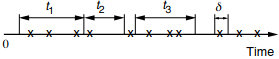
\includegraphics{images/poisson.png}
	\end{center}
\end{figure}


\begin{definition}
	A sequence of arrivals in continuous time is called a Poisson process with rate $\lambda$ if
	\begin{enumerate}
		\item The number of arrivals in disjoint time intervals are independent.
		\item The number of arrivals in an interval of length $\tau$ is given by the Poisson distribution 
		$$
		P(k,\tau) = \frac{(\lambda\tau)^k}{k!}e^{-\lambda\tau}.
		$$
	\end{enumerate}
\end{definition}
The expectation of the number of arrivals $N_\tau$ over an interval of length $\tau$ in a Poisson process is given by $\rm E[N_\tau] = \lambda\tau$.
We also have ${\rm Var}[N_\tau] = \lambda\tau$.

\paragraph{Example: }
Let us assume that the arrivals of golfettes are a Poisson process with 1 golfette arrival every 10 minutes. 
What is the probability of 0, 1, 3 golfette arrivals within half an hour? We have $\lambda \tau = 1/10*30 = 3$
$$
P(0,30) = \frac{3^0}{0!}\times e^{-3} = e^{-3} = 0.05
$$
$$
P(1,30) = \frac{3^1}{1!}\times e^{-3} = 3e^{-3} = 0.15
$$
$$
P(3,30) = \frac{3^3}{3!}\times e^{-3} = e^{-3} = 0.22
$$

Even when a problem makes no mention of Poisson processes, there are sometimes ways to pretend the rvs are coming from a Poisson
process so that we can use convenient Poisson process properties.

\subsection{Arrival times}
Another interesting rv is the one describing the time to the $N$-th arrival. 
Let us denote it $T(n)$.
Notice that $P(T(n)\leq t) = P(N(t)\geq n)$.
Hence, 
\begin{equation}
	P(T(n)\leq t) = 1 - P(N(t)< n) = 1-\sum_{k = 1}^{n-1} \frac{(\lambda t)^k}{k!}e^{-\lambda t}
	= \sum_{k = n}^\infty \frac{(\lambda t)^k}{k!}e^{-\lambda t}
\end{equation}
Moreover, the PDF is obtained by deriving the CDF, which yields
\begin{equation}
	f_{T_n}(t) = \frac{(\lambda t)^{k-1}}{(k-1)!}\lambda e^{-\lambda t}.
\end{equation}
Alternatively, it can be proven using the definition of a density of probability
\begin{equation}
f_{T_n}(t) = \underset{\delta\rightarrow 0}{\rm lim} \frac{P(t<T_n<t+\delta)}{\delta}.
\end{equation}
Notice that for $k=1$, the time of the first arrival is given by the exponential distribution  $f_{T_1}(t) = \lambda e^{-\lambda t}$.

\begin{definition}
	A positive rv $X$ is memoryless if 
	\begin{equation}
		P(X>x_1+x_2) = Pr(X>x_1)Pr(>x_2), \quad\forall x_1,x_2>0.
	\end{equation}
	
	Alternatively, a distribution is said to have the memoryless property if a random variable $X$ from that distribution satisfies
	\[
	P(X \geq s + t \mid X \geq s) = P(X \geq t)
	\]
	for all $s, t > 0$.
\end{definition}
Poisson processes are memoryless. The time to the next arrival is independent of the past.
There are a couple of ways to picture this. 
\begin{enumerate}
	\item 
	The first is the analogy with Bernoulli processes, which at the limit, define Poisson processes. In a Bernoulli process, the outcome of a coin flip does not impact the outcome of the next coin flip.
	\item	The second one if to take a real-world example. Consider phone calls that you get from strangers by mistake. The time at which the phone rings is independent from the previous ones. The process is memoryless. 
\end{enumerate}

\begin{exercise}
	Fishing 
\end{exercise}

\subsection{Conditionning}
Consider a Poisson process with conditionning on the total number
of events in an interval?
\begin{theorem}
	Let $\{N (t), t > 0\}$ be a Poisson process with
	rate $\lambda$, and let $t_1 < t_2$. 
	The conditional distribution of $N(t_1)$ given $N(t_2) = n$
	is
	$N (t_1) | N (t_2) \sim {\rm Bin}(n,t_1/t_2)$.
\end{theorem}
.
\subsection{Merging Poisson processes}
If we take two independent Poisson processes and merge them, we get another Poisson process. 
This follows from the fact that the sum of independent Poissons is Poisson.
\begin{theorem}[Merging]
Let $N_1(t), t > 0$ and $N_2(t), t > 0$ be independent Poisson processes with rates $\lambda_1$ and $\lambda_2$, respectively. 
The mergeed process $N (t) = N_1(t) + N_2(t)$ is a Poisson process with rate $\lambda_1+\lambda_2$.
\end{theorem}
\begin{proof}
	We use the definition of a Poisson process. 
	\begin{itemize}
		\item Arrivals in disjoint intervals are independent in the combined process because
		they are independent in the two individual processes, and the individual processes are independent of each other. 
		\item The PMF of th merged process is given by
		\begin{equation}
			\begin{alignedat}{2}
				P(k,\tau) = \sum_{i=1}^n P_1(i,\tau)P_2(k-i,\tau)
				&= \sum_{i=1}^n \frac{(\lambda_1 \tau)^{i}}{i!}\lambda_1 e^{-\lambda_1 \tau} \frac{(\lambda_2 \tau)^{k-i}}{(k-i)!}\lambda_2 e^{-\lambda_2 \tau}\\
				&= \sum_{i=1}^n\binom{k}{i} \frac{(\lambda_1\tau)^i (\lambda_2\tau)^{k-i}}{k!}e^{-(\lambda_1+\lambda_2) \tau}\\
				&=  \frac{((\lambda_1+\lambda_2) \tau)^k}{k!} e^{-(\lambda_1+\lambda_2)}.
			\end{alignedat}
		\end{equation}
	\end{itemize}
	whereof the result.
	\end{proof}
\paragraph{Question:} What is the probability that the arrival $i$ from one process or the other?
\paragraph{Exercice:} Suppose that student phones running out of charge are exponentially distributed with ditribution ${\rm Exp}(\lambda)$ for each student. We decide not to leave the classroom until the last phone runs out of charge. When would we be able to leave the classroom (on average)?

An exponential rv is the 1st occurrence in a Poisson process. Consider a Poisson process that merges $M$ processes, one for each student. 
The expected time until the 1st phone runs out of charge is $1/(M\lambda)$. 
We are now left with $M-1$ students, and the same number of Poisson processes to merge. 
The expected time until the 2nd phone runs out of charge is $1/((M-1)\lambda)$.
Thus, the expected time at which all phones have ran out of charge
$$
t = \frac{1}{M\lambda}+\frac{1}{(M-1)\lambda}+\ldots+\frac{1}{\lambda}
= \frac{1}{\lambda}\sum_{i=1}^M\frac 1 M.
$$ 
\subsection{Splitting Poisson processes}
Consider a Poisson process.
For each arrival, we independently flip a coin to decide whether it is a type-1 event or type-2 event, we end up with two independent Poisson processes. 
This is the converse of merging.
\begin{theorem}
	Let $\{N (t), t > 0\}$ be a Poisson process with rate
	$\lambda$, and classify each arrival in the process as a type-1 event with probability $p$ and a type-2 event with probability $1 - p$, independently. 
	Then the type-1 events form a Poisson process with rate $\lambda p$, the type-2 events form a Poisson process with rate
	$\lambda (1-p)$, and these two processes are independent.
	\end{theorem}
	
\begin{proof}
	We use the definition of a Poisson process. 
	\begin{itemize}
			\item Arrivals in disjoint intervals are independent in the splitted processes because
		they are independent in the individual parent process.
		\item The PMF of the type-1 splitted process  is given by
		\begin{equation}
			P_1(k,\tau) = p^k  \frac{(\lambda \tau)^{k}}{k!}\lambda e^{-\lambda \tau}
		\end{equation}
		which is the PMF of a Poisson process of rate $\lambda p$; whereof the result.
		\end{itemize}
	
\end{proof}


\newpage
\section{Continuous-Time Markov chains}

\begin{definition}
	A stochastic process $\{ X(t) : t \geq 0 \}$ with discrete state space $S$ is called a continuous-time Markov chain (CTMC) if for all $t \geq 0$, $s \geq 0$, $i \in S$, and $j \in S$,
	$$
	P(X(s + t) = j \mid X(s) = i, \{ X(u) : 0 \leq u < s \}) = P(X(s + t) = j \mid X(s) = i) = P_{ij}(t).
	$$
	$P_{ij}(t)$ is the probability that the chain will be in state $j$, $t$ time units from now, given it is in state $i$ now.
	For each $t \geq 0$, there is a transition matrix
	$$
	P(t) = (P_{ij}(t)).
	$$
\end{definition}



\subsection{Infinitesimal generator}
The infinitesimal generator matrix $\bm Q = (q_{ij})_{1\leq i,j\leq n}$ is given by
\begin{equation}
	q_{ij} = 
	\begin{cases}
		b_{ij},\qquad\qquad	\text{if } j=i+1,\\
		d_{ij},	\qquad\qquad \text{if }  j=i-1,\\
		-b_{ij}-d_{ij}, \quad	\text{if } i=j.	\\
	\end{cases}	
\end{equation}


\subsection{Forward Kolmogorov equation}
On the other hand, the forward Kolmogorov differential equation describes the probability distribution of a state
in time $t$ keeping the initial point fixed. 
It decomposes the time interval $(0,t+s)$ into $(0,t)$ and $(t, t+s)$ by a so-called "last step analysis". 
We differentiate with respect to $t$ then set $t=0$, which yields
\begin{equation}
	p_{ij}'(s) = \sum_{k=1}^n p_{ik}(s)p_{kj}'(0).
\end{equation}
Using the infinitesimal generator, the Kolmogorow backward equation is then given by
\begin{equation}
	\bm P'(s) = \bm P(s)\bm Q 
\end{equation}


\subsection{Backward Kolmogorov equation}
The backward Kolmogorov differential equation describes the transition probabilities in their dependence on the initial point $i$. 
Basically, it analyzes the time interval $(0,t+s)$ by the "first step analysis".
It holds that
$$
p_{ij}(h) = \delta_{ij}+h q_{ij}+o(h).
$$
Thus,
\begin{equation}
	p_{ij}'(0) = \frac{p_{ij}(h)-p_{ij}(0)}{h}
	= q_{ij}.
\end{equation}
The CKE in continuous form is written as
\begin{equation}
	p_{ij}(s+t) = \sum_{k=1}^n p_{ik}(s)p_{kj}(t).
\end{equation}
We differentiate with respect to $s$ then set $s=0$, which yields
\begin{equation}
	p_{ij}'(t) = \sum_{k=1}^n p_{ik}'(0)p_{kj}(t).
\end{equation}
Using the infinitesimal generator, the Kolmogorow backward equation is then given by
\begin{equation}
	\bm P'(t) = \bm Q \bm P(t)
\end{equation}

The Kolmogogrov backward equation i a first order ODE whose solution is given by 
\begin{equation}
	P(t) = e^{\bm Q t} = \sum_{k=1}^\infty \frac{\bm Q^k t^k}{k!}.
\end{equation}


\subsection{Birth-death processes}
A birth-death chain on states $\{1,2,\ldots,M\}$
is a Markov chain with transition matrix $Q = (q_{ij})$ such that $q_{ij} > 0$ if $|i - j| = 1$
and $q_{ij} = 0$ if $|i - j| \geq 2$. 
This says it's possible to go one step to the left and possible to go one step to the right (except at boundaries) and possible to stay in the same state, but impossible to jump further in one step. 
The name stems from applications to the growth or decline of
a population, where a step to the right is thought of as a birth and a step to the left is thought of as a death in the population.
For example, the chain shown below is a birth-death chain if the labeled transitions have positive probabilities, except for the loops from a state to itself, which are allowed to have $0$ probability.
\begin{figure}
	\begin{center}
		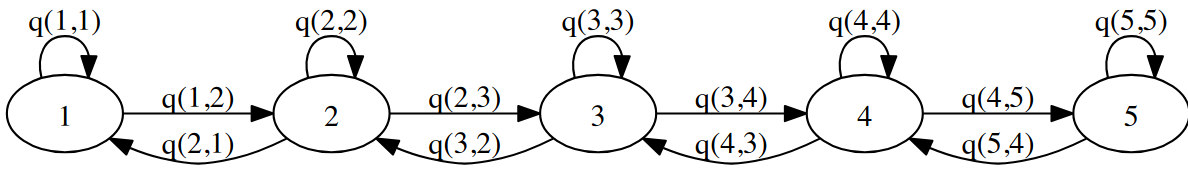
\includegraphics[width =.7\textwidth]{images/birth_death.png}
	\end{center}
\end{figure}
We will now show that any birth-death chain is reversible, and construct the stationary distribution.
A birth death process is an irreducible aperiodic Markov chain. Hence, it has a unique stationary distribution $\bm s$ that is a reversible one.
Reversibility can be shown using the fact that the frequency of moves forward is the same as that of moves backward because in order to move forward $n$ times one needs to have moved backward $n-1$ times at least. Thus long term frequencies of moves forward and backward between two nodes should be equal, i.e,
$$
s_i p_{i(i-1)} = s_{i-1} p_{(i-1)i}\\
$$
$$
s_i = s_{i-1}\frac{ p_{(i-1)i}}{p_{i(i-1)}}
=  s_{i-2} \frac{p_{(i-2)(i-1)}}{p_{(i-1)(i-2)}} \frac{p_{(i-1)i}}{p_{i(i-1)}}
$$
Hence
$$
s_i = s_0\frac{\Pi_{k=1}^{i}p_{(k-1)k}}{\Pi_{k=1}^{i}p_{k(k-1)}}
$$
We retrieve $s_0$ using the property $\sum_i s_i = 1$.

Suppose $p_{i(i+1)}=p$ and $p_{(i+1)i}=q$ for all $i\geq 1$, then 
$$
s_i =s_0 (p/q)^i = s_0 \rho^i,
$$
Using $\sum_{i=0}^n s_i = 1$ yields $s_0 = {1-\rho}$, then $s_i = \rho^i(1-\rho)$.


\subsection{Holding times}
For each state $i \geq 0$ we have a birth rate $\lambda_i$ and a death rate $\mu_i$.
Whenever $X(t) = i$, independent of the past, the time until the next birth is a r.v. $X \sim \text{exp}(\lambda_i)$ and, independently, the time until the next death is a r.v. $Y \sim \text{exp}(\mu_i)$. 
Thus, the holding time rates are given by $a_i = \lambda_i + \mu_i$ because the time until the next transition (change of state) is given by the holding time $H_i = \min\{ X, Y \} \sim \text{exp}(\lambda_i + \mu_i)$. 
The idea here is that at any given time, the next birth is competing with the next death to be the next transition. (We always assume here that $\mu_0 = 0$ since there can be no deaths without a population.)
This means that whenever $X(t) = i \geq 1$, the next transition will be a birth with probability
$$
P_{i,i+1} = P(X < Y) = \frac{\lambda_i}{\lambda_i + \mu_i},
$$
and a death with probability
$$
P_{i,i-1} = P(Y < X) = \frac{\mu_i}{\lambda_i + \mu_i}.
$$
Thus, the embedded chain for a B\&D process is a simple random walk with state-dependent "up" and "down" probabilities.

When $\mu_i = 0$, $i \geq 0$, and $\lambda_i > 0$, $i \geq 0$, we call the process a \textit{pure birth process}; the population continues to increase by one at each transition.


\subsection{Explosion}
Consider a pure birth process $\{ X(t) \}$, $P_{i,i+1} = 1$, $i \geq 0$, in which $a_i = \lambda_i = 2^i$, $i \geq 0$. 
This process spends, on average, $E(H_i) = \frac{1}{\lambda_i} = 2^{-i}$ units of time in state $i$ and then changes to state $i + 1$. 
Thus, it spends less and less time in each state, consequently jumping to the next state faster and faster as time goes on. 
Since $X(t) \to \infty$ as $t \to \infty$, we now explore how fast this happens. 

Note that the chain will visit state $i$ at time $H_0 + H_1 + \cdots + H_{i-1}$, the sum of the first $i$ holding times. 
Thus, the chain will visit all of the states by time
$$
T = \sum_{i=0}^{\infty} H_i.
$$
Taking the expected value yields
$$
E(T) = \sum_{i=0}^{\infty} 2^{-i} = 2 < \infty,
$$
and we conclude that on average all states $i \geq 0$ have been visited by time $t = 2$, a finite amount of time! But this implies that with probability 1, all states will be visited in a finite amount of time; $P(T < \infty) = 1$. 
Consequently, with probability 1, $X(T + t) = \infty$, $t \geq 0$. This is an example of an explosive Markov chain: The number of transitions in a finite interval of time is infinite.
A non-explosive CTMC is one for which the number of
transitions in any finite interval of time is finite.

   \bibliographystyle{plain}
  \bibliography{bibli}
  
  http://www.stat.yale.edu/Courses/1997-98/101/ranvar.htm
  (Definitions taken from Valerie J. Easton and John H. McColl's Statistics Glossary v1.1) 
  
  %CTMC section is from Columbia + nyu syllabi
  
  $file:///home/benaceur/Documents/course_stochastic_processes/markov_cermics.pdf$
  %john tsilsikis
  \end{document}
